\documentclass[conference]{IEEEtran}
\IEEEoverridecommandlockouts
\usepackage[colorlinks=true, urlcolor=blue, linkcolor=red]{hyperref}
\usepackage{amsmath,amssymb,amsfonts}
\usepackage[spanish]{babel}
\usepackage{algorithmic}
\usepackage{multicol}
\usepackage{booktabs}
\usepackage{graphicx}
\usepackage{textcomp}
\usepackage{xcolor}
\usepackage{array}
\usepackage{cite}
\usepackage{url}

\def\BibTeX{{\rm B\kern-.05em{\sc i\kern-.025em b}\kern-.08em
  T\kern-.1667em\lower.7ex\hbox{E}\kern-.125emX}}
\begin{document}

\title{Pruebas sobre el comportamiento de la memoria caché}


\author{\IEEEauthorblockN{Fernando Ramirez Arredondo}
\IEEEauthorblockA{\textit{Computer Science} \\
\textit{Universidad Católica San Pablo}\\
Arequipa, Perú \\
fernando.ramirez@ucsp.edu.pe}}

\maketitle

\begin{IEEEkeywords}
  Caché
\end{IEEEkeywords}

\section{Introducción}\label{sec:intro}
El análisis de algoritmos en términos de uso de recursos es fundamental en computación. En este informe, se analiza comportamiento de la memoria caché mediante la ejecución de dos experimentos, una comparación de rendimiento en bucles anidados y una comparación entre una implementación de la multiplicación de matrices clásica utilizando tres bucles anidados y la implementación de la multiplicación de matrices por bloques, que emplea seis bucles anidados.

La evaluación de las implementaciones se llevará a cabo utilizando diferente tamaño de matrices con el fin analizar cómo el rendimiento varía con el incremento del tamaño del problema. Se utilizarán las herramientas de análisis de rendimiento Valgrind y KCachegrind para obtener una evaluación detallada.

Sección \ref{sec:meto}. presenta la implementación, 
Sección \ref{sec:res}. presenta los resultados, 
Sección \ref{sec:conc}. presenta las conclusiones. 

\section{Implementación}\label{sec:meto}
La implementación de los experimentos fue realizada en C++ usando una maquina virtual Ubuntu 64-bit Arm 22.04.4 con 4 GB de RAM y gcc version 11.4.0. Todo el código fuente se encuentra en el siguiente repositorio online \href{https://github.com/fernandoramirez1337/cache_test/tree/main}{GitHub}.
\subsection{Bucles anidados}
Se midió el tiempo de ejecución de cada implementación con listas de 64, 128, 256 y 512 elementos.
\subsection{Multiplicaciones de matrices}
Se midió el tiempo de ejecución con matrices de tamaños 64x64, 128x128, 256x256 y 512x512. La implementaciones de bloques fue realizada con un bloque de tamaño 4, tras comparar tiempo de ejecución con bloques de tamaño 2, 4, 8 y 16.

\section{Resultados}\label{sec:res}
Esta sección presenta los resultados encontrados, apoyandose de la teoría del libro referencia del curso. 
\subsection{Bucles anidados}
\begin{figure}
  \centering
  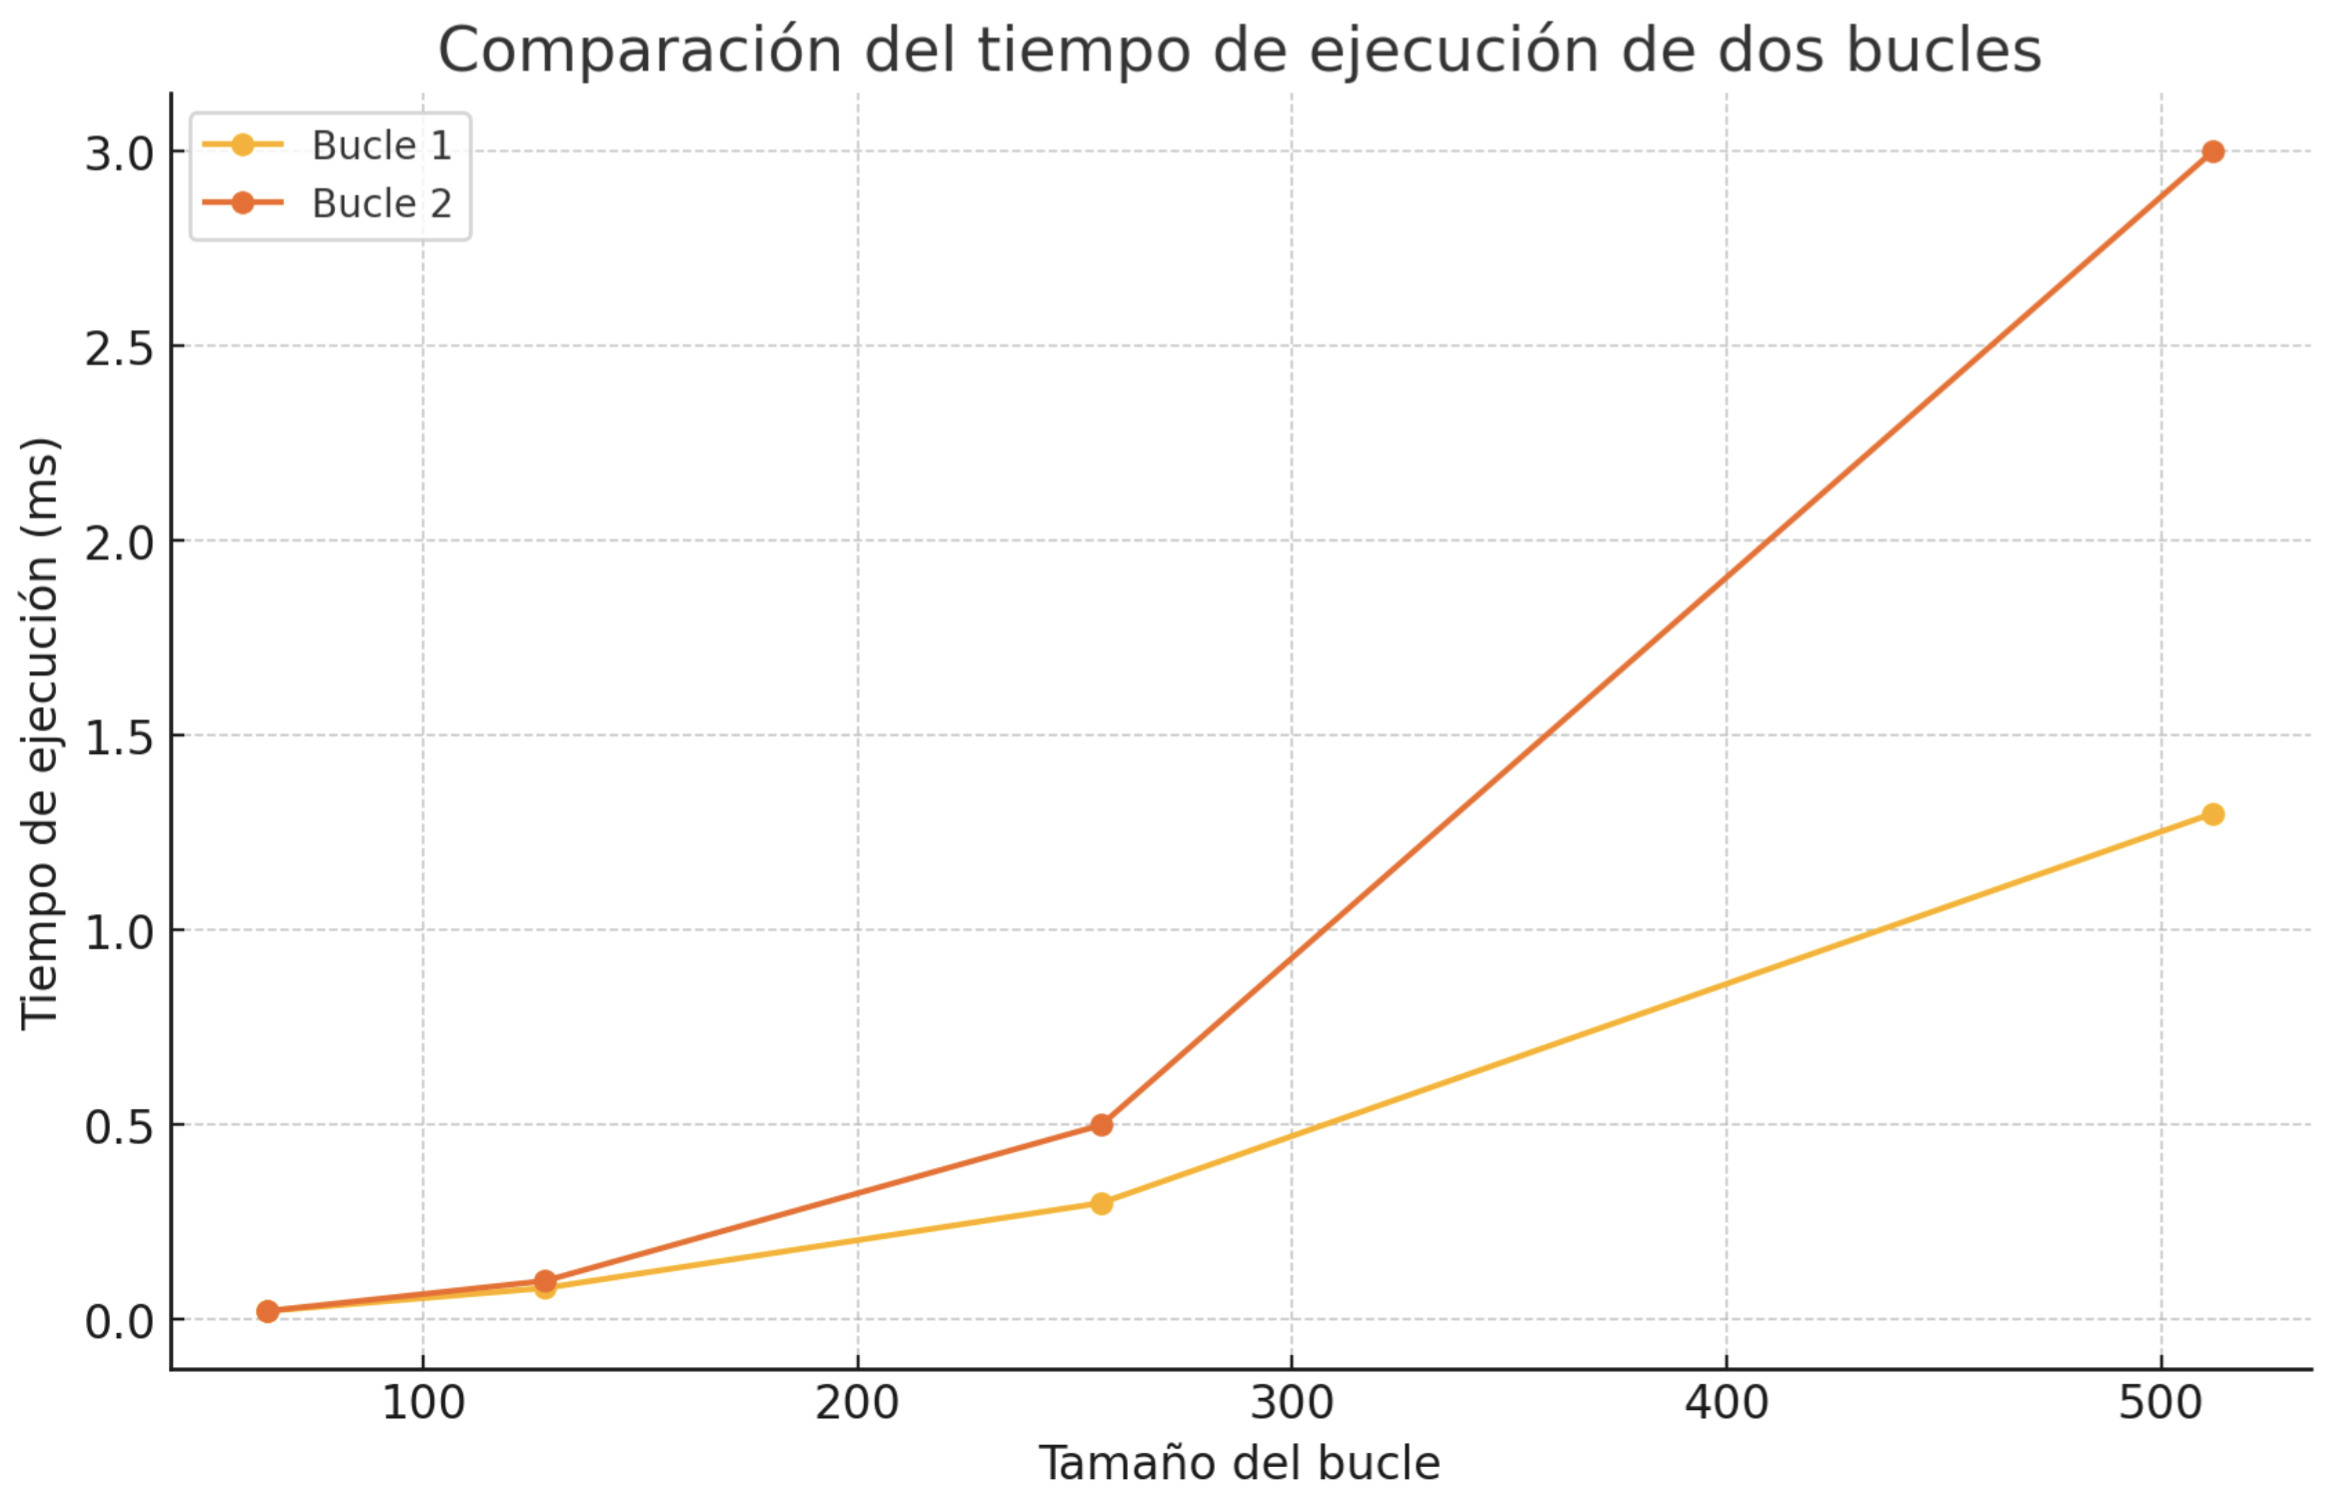
\includegraphics[width=\columnwidth]{figures/bucles.png}
  \caption{Comparación de tiempo de ejecución de ambos bucles con diferente número de datos.}
  \label{fig:bucles}
\end{figure}
En la Fig. \ref{fig:bucles} se observa que el primer bucle (j interior, i exterior) es el más rápido de los dos. El segundo bucle (j exterior, i interior) demora más tiempo en ejecutarse con cada uno de los diferentes tamaños, teniendo peor desempeño con las dimensiones más altas. En terminos de caché, el segundo bucle es ineficiente ya que accede a la matriz A en un orden de columna mayor, que es ineficiente en sistemas que almacenan matrices en orden de fila mayor. Esto conduce al acceso a ubicaciones de memoria no adyacentes, lo que resulta en más errores de caché y mayor tiempo de ejecución.\cite{pacheco2011introduction}

\subsection{Multiplicaciones de matrices}
\begin{figure}
  \centering
  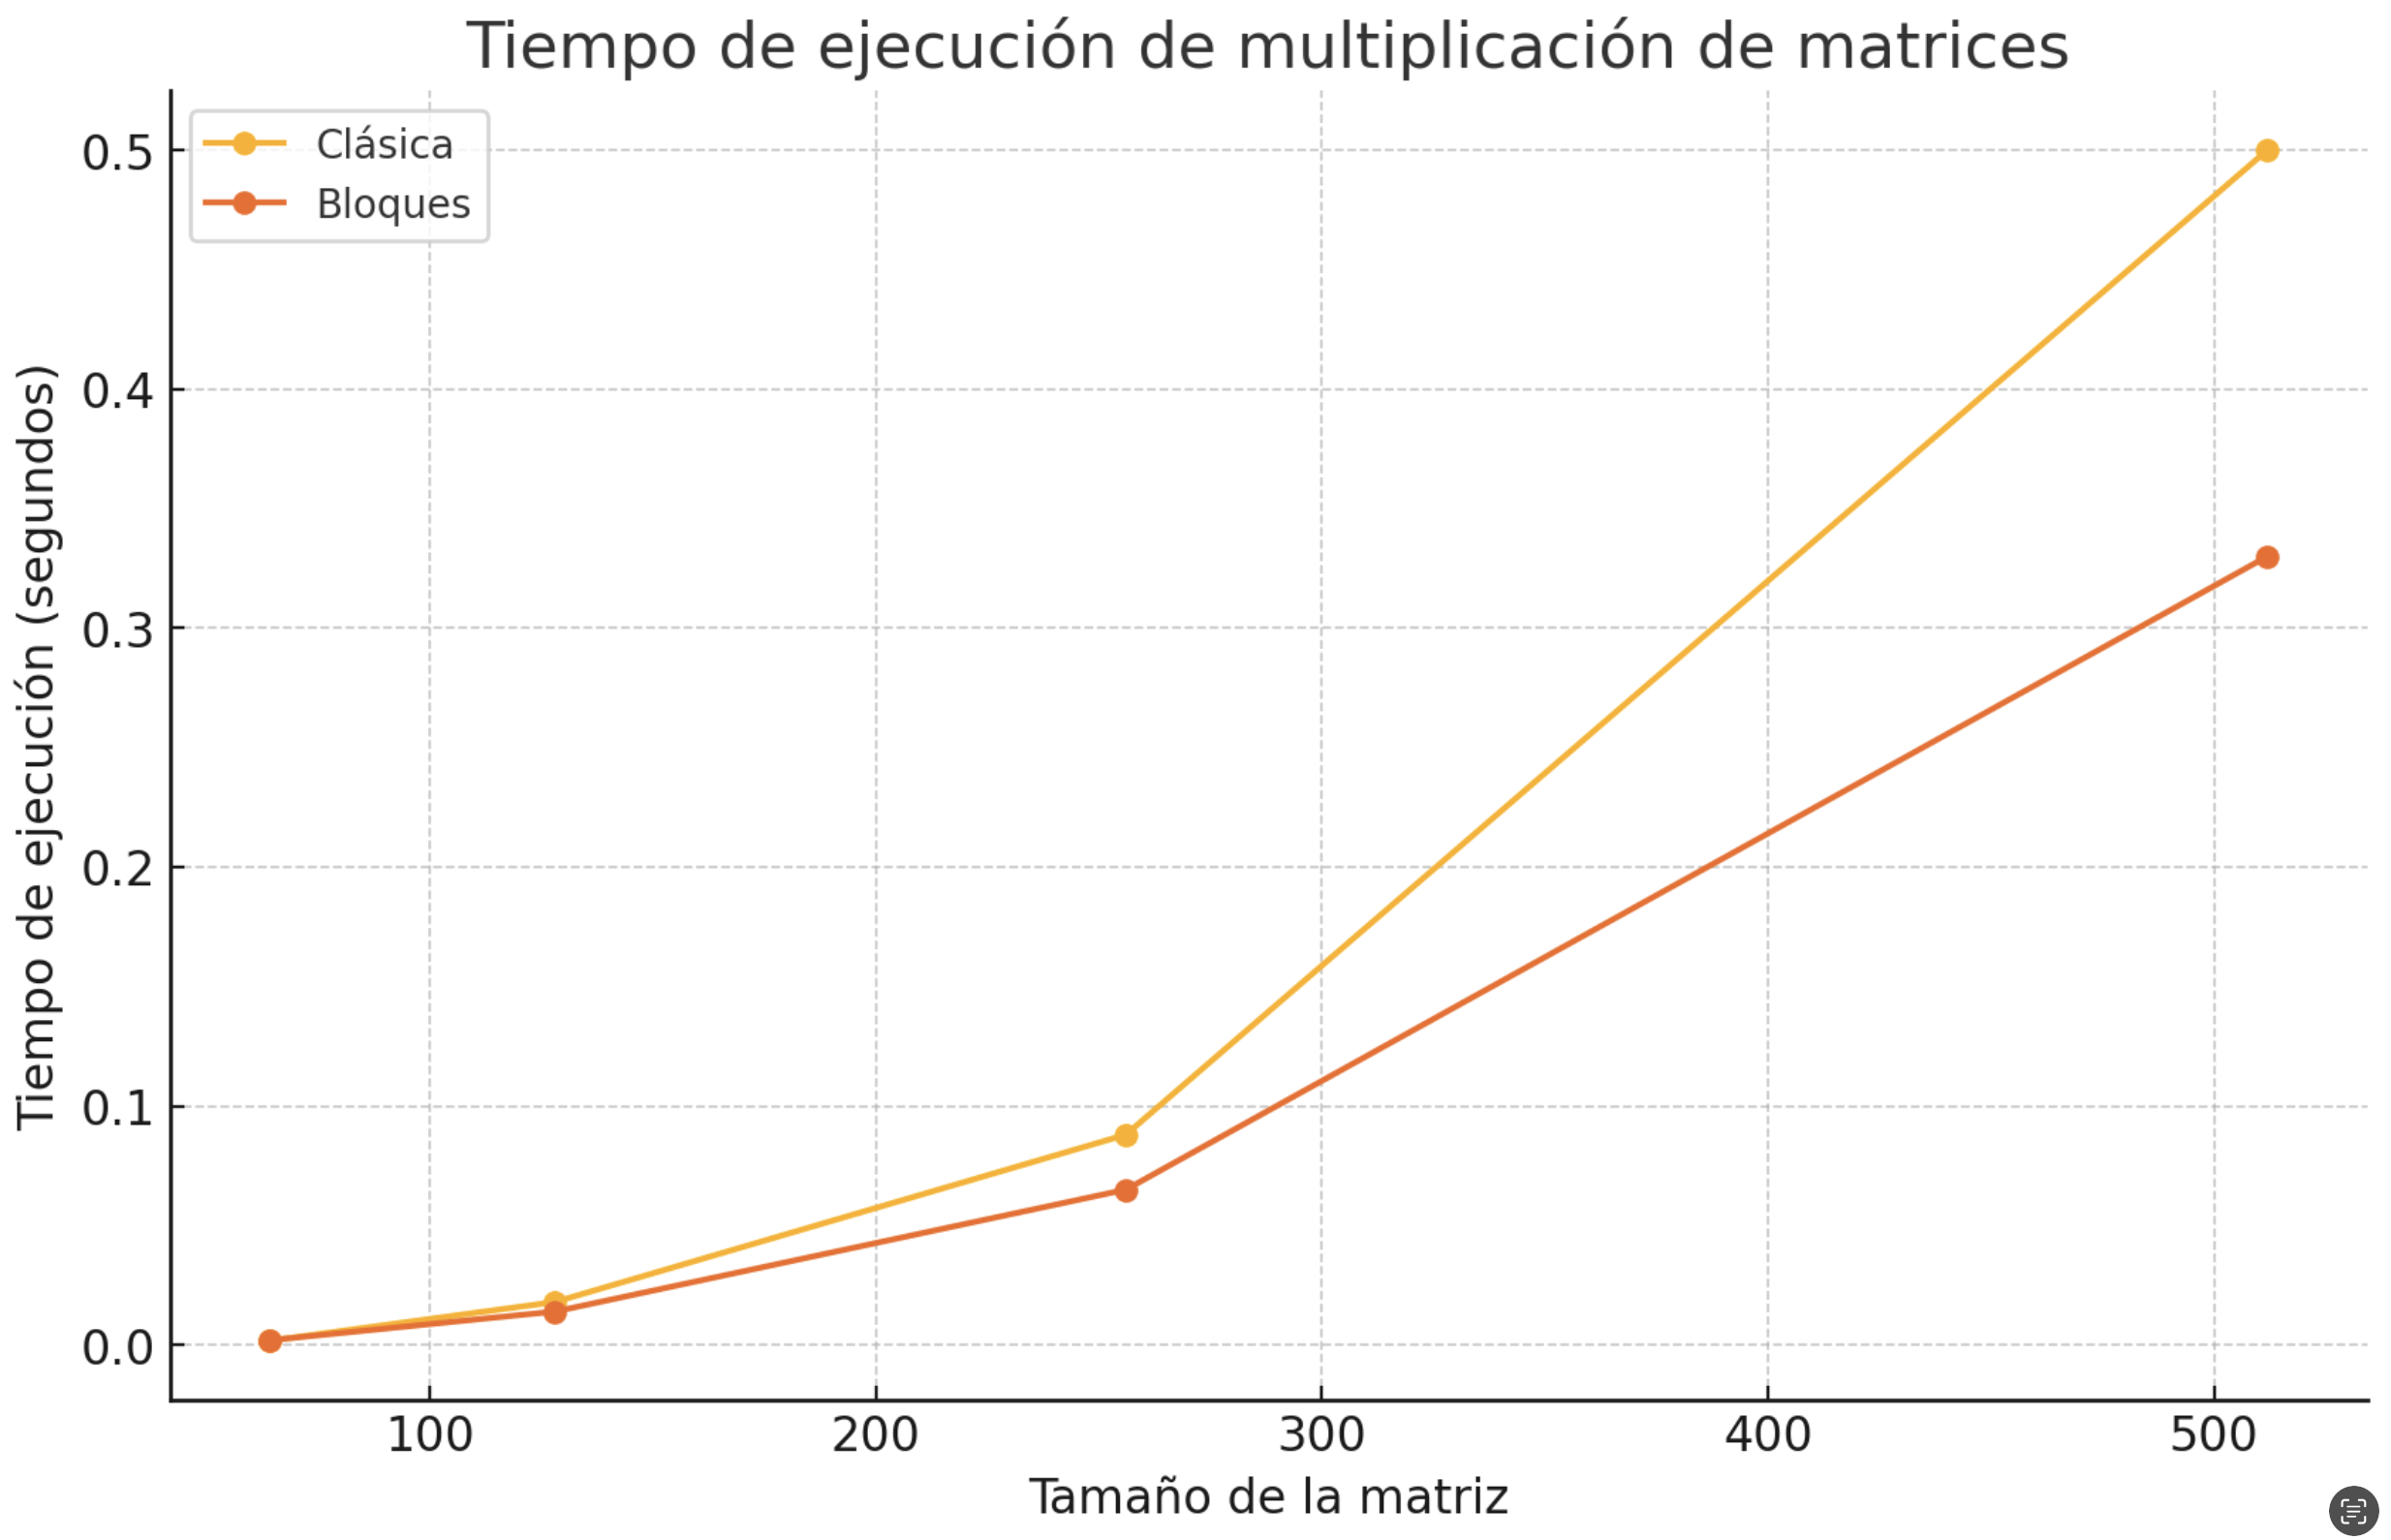
\includegraphics[width=\columnwidth]{figures/matrices.png}
  \caption{Comparación del tiempo de ejecución de ambas multiplicaciones con diferente número de datos.}
  \label{fig:matrices}
\end{figure}
En la Fig. \ref{fig:matrices} se observa que la multiplicación de matrices por bloques tiene mejor desempeño que la version clásica de tres bucles. Utilizando Valgrind y KCachegrind se observa que la implementación por bloques realiza 5 millones de instrucciones y la implementación clásica realiza 4 millones de instrucciones con matrices de tamaño 512x512. La implementación por bloques es más rápida que la clásica, a pesar de ejecutar un mayor número de instrucciones, debido a la optimización del uso de la caché de la CPU, La multiplicación por bloques explota mejor la localidad espacial y temporal de los datos. La localidad espacial se refiere a que los elementos cercanos en la memoria tienden a ser accedidos juntos, y la localidad temporal se refiere a que los datos que se han accedido recientemente tienen más probabilidades de ser accedidos de nuevo en breve mientras que la multiplicación clásica accede a los elementos de las matrices de manera que genera muchos fallos de caché.\cite{pacheco2011introduction}
\section{Conclusiones}\label{sec:conc}
El análisis de los experimentos realizados demuestra la importancia del orden de acceso a la memoria y la organización de los datos en el rendimiento de algoritmos.

En el caso de los bucles anidados, se confirmó que el orden de acceso influye significativamente en el desempeño, donde el acceso a la matriz en orden de fila mayor resultó en menos errores de caché y tiempos de ejecución más bajos. Este resultado muestra la necesidad de considerar la organización de los datos y el orden de los bucles en la optimización de código.

Para la multiplicación de matrices, se observó que la técnica de bloques, a pesar de ejecutar un mayor número de instrucciones, supera en rendimiento a la multiplicación clásica. Esto se debe a la mejora en la localidad espacial y temporal, lo que optimiza el uso de la caché y reduce los errores de caché. Ambas implementaciones tienen una complejidad de $O(n^3)$, sin embargo, la implementación por bloques muestra un mejor rendimiento práctico debido a la reducción en los errores de caché, lo que destaca la diferencia entre la complejidad teórica y el rendimiento real en un entorno con limitaciones de memoria.

La implementación de técnicas que consideren la arquitectura del computador puede llevar a mejoras significativas en sistemas donde la eficiencia en el acceso a la memoria es crucial para el rendimiento, especialmente en el contexto de la memoria caché.

Repositorio online:
\href{https://github.com/fernandoramirez1337/cache_test/tree/main}{github.com}.



\bibliographystyle{IEEEtran}
\bibliography{bibliography/references}
\vspace{12pt}

\end{document}